\documentclass[11pt]{beamer}

%http://mirrors.ibiblio.org/CTAN/macros/latex/contrib/beamer-contrib/themes/metropolis/doc/metropolistheme.pdf
\usetheme[progressbar=frametitle, subsectionpage=progressbar, sectionpage=none]{metropolis}
\usepackage{appendixnumberbeamer}
\usepackage{multirow}
\usepackage{makecell}
\usepackage{adjustbox}
\usepackage{tabularx}

\usepackage{booktabs}
\usepackage[scale=2]{ccicons}

\usepackage{pgfplots}
\usepgfplotslibrary{dateplot}

\usepackage{tikz}
\usetikzlibrary{arrows,positioning,shapes.misc} 

\usepackage{xspace}

%\definecolor{mDarkBrown}{HTML}{604c38}
\definecolor{mDarkTeal}{HTML}{233350} %% orig: 23373b -- changed to match UP logo colour
%\definecolor{mLightBrown}{HTML}{EB811B}
%\definecolor{mLightGreen}{HTML}{14B03D}

\usepackage[backend=biber, 
		natbib=true, 
		style=C:/texmf/bst/biblatex-sp-unified/bbx/biblatex-sp-unified,
		citestyle=C:/texmf/bst/biblatex-sp-unified/cbx/sp-authoryear-comp, 
		maxbibnames=99, 
		isbn=false, 
		doi=false, 
		eprint=false]{biblatex}
\addbibresource{ep.bib}
\setbeamertemplate{bibliography item}{}  %% To stop a little icon appearing.

% -------------------------------------

%% Creates a description environment where the text for each item is evenly
%% left-aligned based on the width of the longest label.
%% Source: https://tex.stackexchange.com/questions/23559/how-to-control-enumitems-description-list-via-leftmargin-and-labelwidth-keys
\newenvironment{mydesc}[1]
{\list{}{\renewcommand\makelabel[1]{\textbf{##1}\hfil}%
		\settowidth\labelwidth{\makelabel{#1}}%
		\setlength\leftmargin{\dimexpr\labelwidth+\labelsep\relax}}}
{\endlist}

%% Changes the beamer template to have the total slides displayed as well as
%% the current slide.
\setbeamertemplate{footline}{% 
	\hfill% 
	\usebeamercolor[fg]{page number in head/foot}% 
	\usebeamerfont{page number in head/foot}% 
	\insertframenumber\,/\,\inserttotalframenumber
	\kern1em\vskip15pt
}

\setbeamercolor{background canvas}{bg=white}

% -------------------------------------

\newcommand{\sfx}[1]{\mbox{-\textit{#1}}}
\newcommand{\pfx}[1]{\mbox{\textit{#1}-}}

\newcommand{\hkeit}{\mbox{-\textit{heit}}/\mbox{-\textit{keit}}\xspace}
\newcommand{\pp}{$\mathscr{P}$\xspace}

\newcommand{\hfillcite}[1]{ {\color{mDarkBrown} {\scriptsize \hfill\citep{#1} }} }

% -------------------------------------

\definecolor{firanavy}{RGB}{0,0,139}
\definecolor{firateal}{RGB}{73,146,147}
\definecolor{firagold}{RGB}{226, 189, 54}

% -------------------------------------

\title{Taboo implementation}
\subtitle{BM1 Advanced NLP -- Final project}
\date{February 6, 2020}
\author{Anna-Janina Goecke, \newline Rodrigo Lopez Portillo Alcocer, \newline Elizabeth Pankratz \newline}
\institute{Universität Potsdam}
 \titlegraphic{\vspace{0.25cm}\hfill
\includegraphics[height=2cm]{01_UP.jpg}}

% -------------------------------------

\begin{document}
	
\maketitle

% -------------------------------------

\begin{frame}{Our goal}

\begin{columns}

\begin{column}{0.5\textwidth}

	\begin{center}
		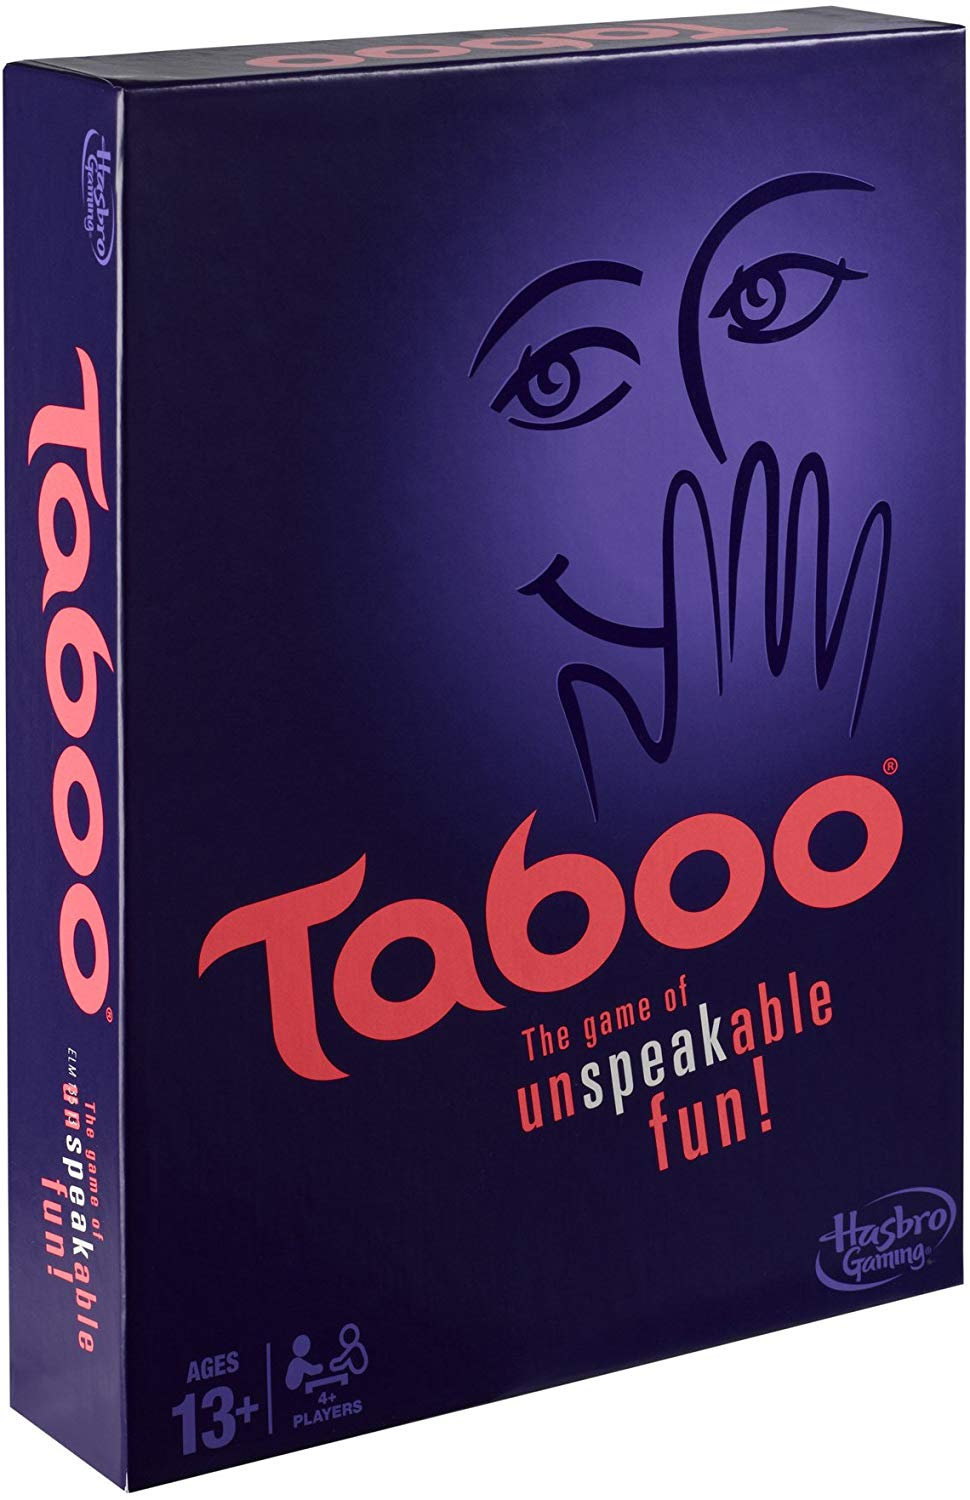
\includegraphics[width=.6\linewidth]{taboo.jpg}
	\end{center}
		
	\vfill 
	{\tiny \href{https://www.amazon.com/Hasbro-A4626-Taboo-Board-Game/dp/B00D4NJSBW}{(image source)} }

\end{column}

\begin{column}{0.5\textwidth}

	We are implementing two components of the gameplay:
	
	\begin{itemize}
		\item[$\rightarrow$] \textbf{Taboo card generator}
		\begin{itemize}
			\item pre-trained word2vec word embeddings
			\item WordNet via NLTK
		\end{itemize}
		\item[$\rightarrow$] \textbf{Taboo player}
		\begin{itemize}
			\item LSTM RNN using PyTorch
		\end{itemize}
	\end{itemize}

\end{column}
	
\end{columns}

\end{frame}

% -------------------------------------

\begin{frame}{Part 1: The card generator}

\begin{columns}
	
	\begin{column}{0.5\textwidth}


	\begin{enumerate}
		\item \textbf{Gold standard} from existing Taboo cards
		\begin{itemize}
			\item semantic relations manually annotated
		\end{itemize}
		\item \textbf{Taboo word generation} for a given main word
		\begin{itemize}
			\item five words based on probability distribution from gold standard
		\end{itemize}
	\end{enumerate}

	\end{column}
	
	\begin{column}{0.5\textwidth}
		
		
		\begin{center}
			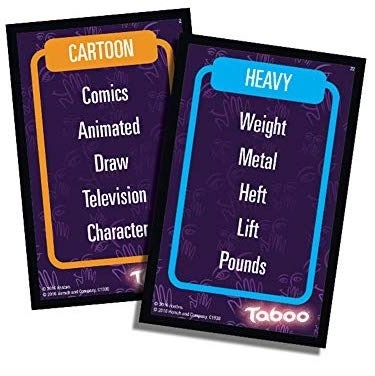
\includegraphics[width=.9\linewidth]{cards.jpg}
		\end{center}

		\hfill {\tiny \href{https://www.amazon.com/Hasbro-Gaming-Buzzer-Amazon-Exclusive/dp/B06XYL6Y5C}{(image source)} }
		
	\end{column}


	
\end{columns}

\end{frame}

% -------------------------------------

\begin{frame}[fragile]{Part 1: The card generator}



\begin{columns}
	
\begin{column}{0.65\textwidth}

\begin{center}
	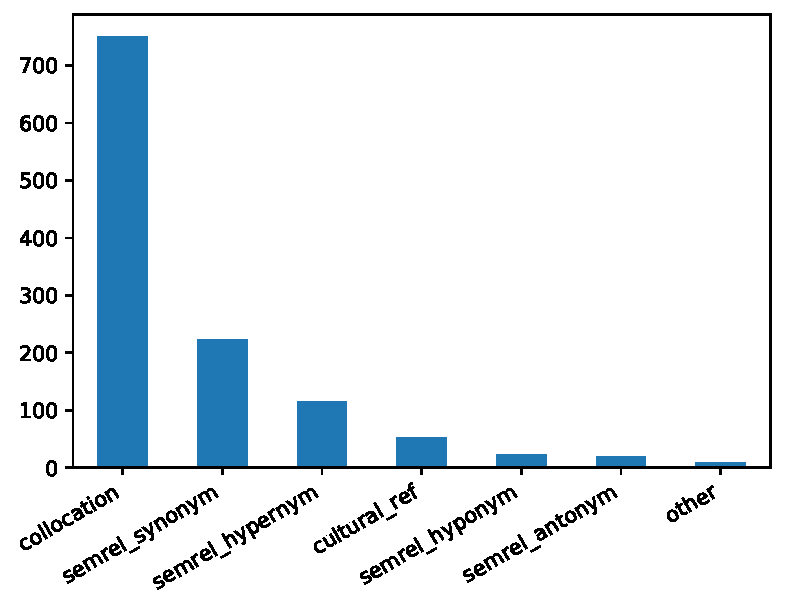
\includegraphics[width=\linewidth]{freq_plot.pdf}
\end{center}

\end{column}

\begin{column}{0.35\textwidth}

\vspace{-\baselineskip}

{\scriptsize
\begin{semiverbatim}
---------------------
|   taboo           |
---------------------
|   stigma          |
|   verboten        |
|   touchy          |
|   forbidden       |
|   unmentionable   |
---------------------
\end{semiverbatim}
}
\end{column}

\end{columns}

\end{frame}


% ----------------------------------------------


\begin{frame}{Part 2: The Taboo player}
	
	\begin{itemize}
		\item NN to generate text (RNN with LSTM architecture)
		\item Idea: start with e.g.\ ``a [main word] is a'' to get NN on the right track
		\item Implementation using PyTorch
	\end{itemize}
	
\end{frame}

% ----------------------------------------------

%\appendix
%
%\begin{frame}[allowframebreaks]{References}
%
%\renewcommand*{\bibfont}{\tiny}
%\printbibliography
%
%\end{frame}

% ----------------------------------------------

\end{document}